\lab{Algorithms}{Newton-Cotes Integration}{Newton-Cotes Integration}

\objective{Explain Newton-Cotes Integration}

One of the fundamental problems in calculus is integration. However, in the vast majority of cases it is impossible to integrate functions analytically. In these cases our only option is to approximate the integral numerically.

One of the most natural approaches is to use the trapezoidal rule. This approach approximates the integral of a function by using the average of its values at the left and right endpoints of the interval of integration:
\[
\int_a^b f(x) dx \approx (b-a)\frac{f(a) + f(b)}{2}
\]

This approach is equivalent to approximating the integral by integrating the linear interpolant of the function. For an illustration see Figure \ref{Fig:Trapezoidal}

\begin{figure}
\begin{center}
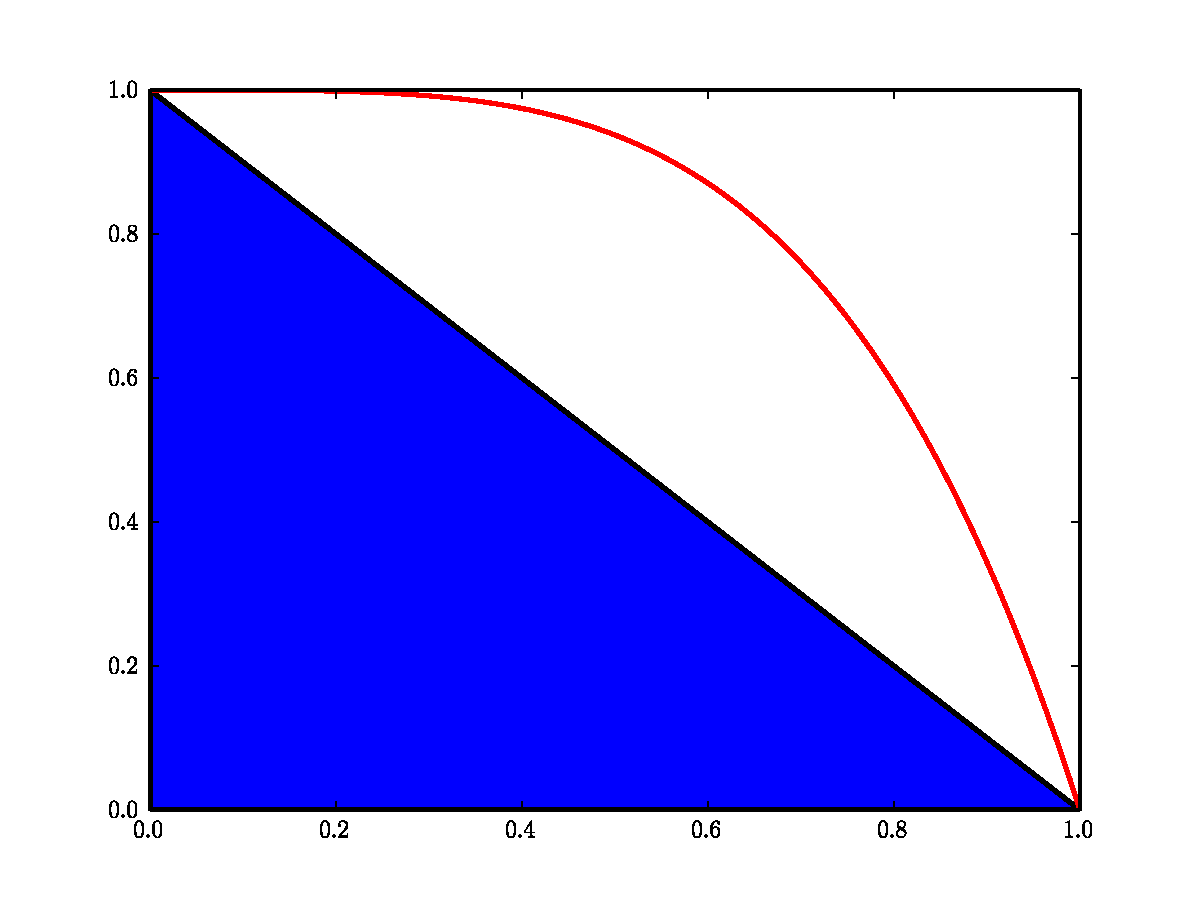
\includegraphics[scale=.4]{Trapezoid.pdf}
\caption{Demonstration of approximating the integral $\int_0^1 (1-x^4)dx$ using the trapezoidal rule. The shaded area is the area approximated by the trapezoidal rule, and the actual function is given in red.}
\label{Fig:Trapezoidal}
\end{center}
\end{figure}

A few questions rise naturally about the trapezoidal rule. The first is, how good is our approximation? It turns out, that for a twice differentiable function the error is equal to:
\[
\mbox{error} = \frac{(b-a)^3}{12}f^{(2)}(\xi) \mbox{ where } \xi \in [a,b]
\]
Thus, the error is proportional to both $(b-a)^3$ and the second derivative. The fact that the error is proportional to the value of the second derivative makes sense: the trapezoidal rule cannot compensate for a function having non-zero second derivative.

How can we more accurately approximate the integral of a function? One technique is to break our interval into many smaller sub-intervals. This is known as a \emph{composite rule}. We will delay discussion of composite rules momentarily and discuss a different approach first.

Note that the trapezoidal rule is really just approximating the integral by integrating the linear interpolant of the function. Suppose instead that we approximate our function with a higher-order interpolant. We can write this method mathematically as follows:
\[
\int_a^b f(x) dx \approx \int_a^b \sum_{j=1}^n L_j(x)f(x_j) dx = \sum_{j=1}^n f(x_j)\int_a^b L_j(x) dx
\]

We can analytically pre-compute the value of $w_j = \int L_j(x)$ for a given set of interpolation points $\{x_j\}$ and thus write our approximation as
\[
\int_a^b f(x) dx \approx \sum_j w_j f(x_j)
\]

A set of points $x_j$ and corresponding weights $w_j$ are known as a \emph{quadrature rule}. In this Lab we will focus on evenly-spaced points $x_j$, and in Lab \ref{Lab:GaussQuad} we will look at other sets of points.

Note that this method will exactly integrate polynomials of order $n-1$ (where $n$ is the number of points). This is because the polynomial interpolant ($\sum L_j f(x_j)$) will exactly match the function $f$.

Using three evenly-spaced points we can (using a little algebra) derive the following integration rule:
\[
\int_a^b f(x) dx \approx \frac{(b-a)}{6}\left(f(x_1) + 4 f(x_2) + f(x_3)\right)
\]

This is known as \emph{Simpson's Rule}. We can implement Simpson's rule in Python as follows:
\begin{lstlisting}
: def SimpsonsRule(func, a, b):
....: return ((b-a)/6.0)*sp.array([1,4,1])*func(sp.vstack([a,(b-a)/2.0,b]))
\end{lstlisting}


We can test this function on $\sin(x)$ as follows:
\begin{lstlisting}
: import scipy as sp
: SimpsonsRule(sp.sin, 0, sp.pi)
array([[  0.00000000e+00,   0.00000000e+00,   0.00000000e+00],
       [  5.23598776e-01,   2.09439510e+00,   5.23598776e-01],
       [  6.41202387e-17,   2.56480955e-16,   6.41202387e-17]])
\end{lstlisting}


The answer, which we can find analytically, is $2$. For only evaluating the function at three points this is fairly accurate.

\begin{problem}
Two higher-order quadrature rules are the Simpson 3/8 rule and Boole's rule. They can be written in the following formulae:
\begin{align*}
\int_a^b f(x) dx &\approx \frac{(b-a)}{8}\left(f(x_1) + 3 f(x_2) + 3 f(x_3) + f(x_4)\right) \\
\int_a^b f(x) dx &\approx \frac{(b-a)}{90}\left(7f(x_1) + 32 f(x_2) + 12 f(x_3) + 32f(x_4) + 7 f(x_5)\right) \\
\end{align*}

Write a function that implements these quadrature rules. Allow the user to optionally specify which quadrature rule to use.
\end{problem}

Another tool of great importance in numerical integration is composite quadrature rules. These rules break up the interval into many smaller sub-intervals. A desired quadrature rule is then applied to each sub-interval, and the results are summed together. Mathematically we can write such an approach as follows:
\[
\int_a^b f(x) dx = \sum_{i=0}^n \int_{x_i}^{x_{i+1}} f(x) dx
\]
where $a = x_0 < x_1 < \ldots < x_n = b$. We then apply some rule (such as Simpson's rule, or the trapezoid rule) to each smaller integration problem. A graphical illustration of such an approach is shown in Figure \ref{Fig:TrapezoidalComposite}

\begin{figure}
\begin{center}
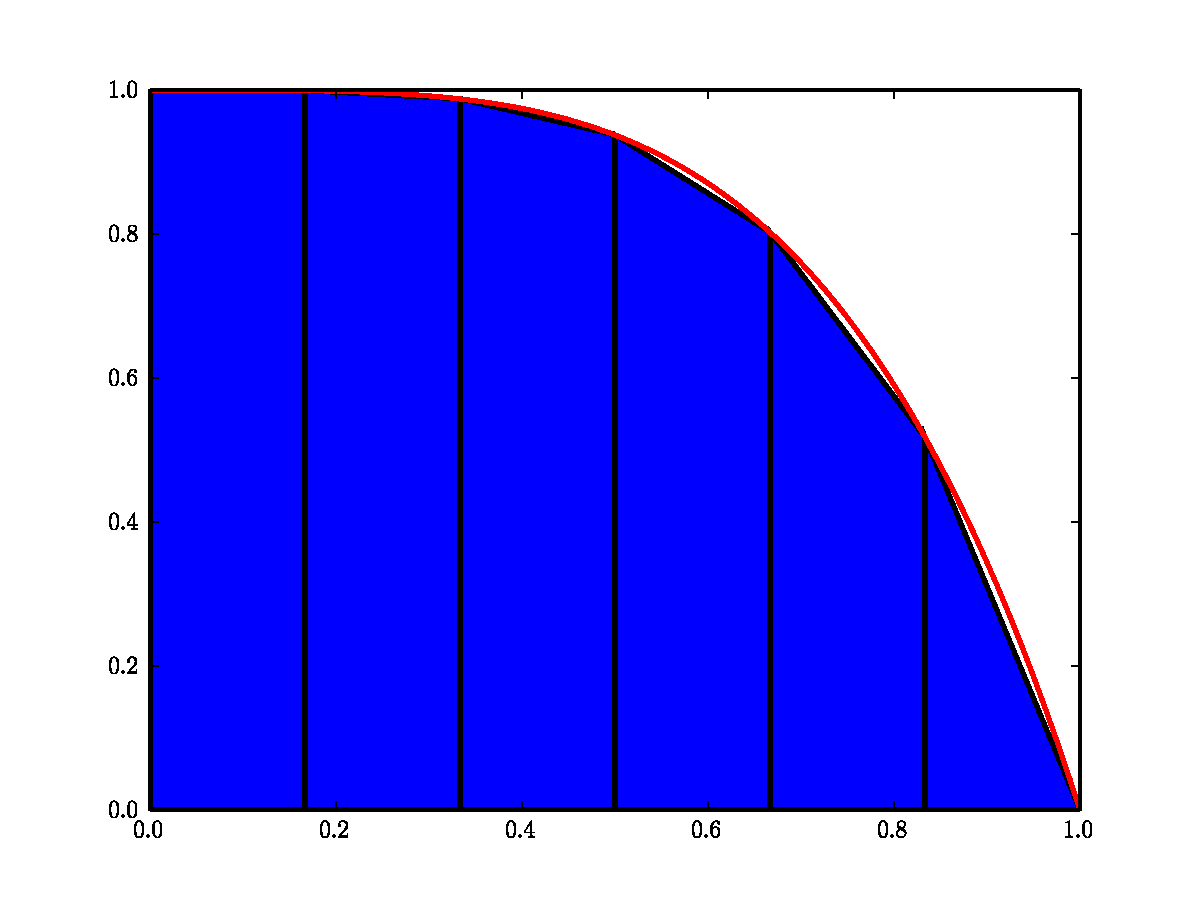
\includegraphics[scale=.4]{TrapezoidComp.pdf}
\caption{Demonstration of approximating the integral $\int_0^1 (1-x^4)dx$ using a composite trapezoidal rule. The shaded area is the area approximated by the composite rule, and the actual function is given in red.}
\label{Fig:TrapezoidalComposite}
\end{center}
\end{figure}

Let's look at how the composite Simpson's rule would work. We divide our interval of integration into $n$ sub-intervals (and thus we have $n+1$ interval endpoints). To use Simpson's rule on each sub-interval we will need the $n$ midpoints of each subinterval. Thus we have points $x_1 \ldots x_{2n+1}$. Of these points, the midpoints are precisely the even indices. Now recall that Simpson's Rule is:

\[
\int_a^b f(x) dx \approx \frac{(b-a)}{6}\left(f(x_1) + 4 f(x_2) + f(x_3)\right)
\]

Applying this to each sub-interval we get the following:
\[
\int_a^b f(x) dx \approx \frac{(b-a)}{6n}\left( f(x_1) + \sum_{i=1}^{n} 4*f(x_{2i}) + \sum_{i=0}^{n-2} 2*f(x_{1+2i}) + f(x_{2n+1})\right)
\]

The initial constant is because each sub-interval has width $(b-a)/6n$. The different weights on each function evaluation $f(x_i)$ are justified as follows: each sub-interval midpoint gets weight of four by Simpson's rule, and sub-interval endpoints that aren't either $a$ or $b$ get counted twice because they belong to sub-intervals to their left and right.

\begin{problem}
Derive the composite rule for Simpson's 3/8 rule and Boole's rule. Implement all three composite rules in a MATLAB function. Require the user to input a maximum sub-interval width. Now test your function by integrating $x^{1/3}$ on the interval $[0,1]$ (which you can analytically solve). Use a log plot to estimate the exponent of convergence for Simpson's Rule and Simpson's 3/8 Rule. You should get roughly the same exponent of convergence (this does not mean that the errors are the same, just that the rate of convergence is the same). Since the two rules have the same exponent of convergence, but the 3/8 rule requires more function evaluations to achieve a similar degree of accuracy, the 3/8 rule is typically not used.
\end{problem}

One other important technique is what is known as \emph{Adaptive Quadrature}. It is clear in Figure \ref{Fig:TrapezoidalComposite} that we have approximated the integral better in some places than in others. In fact on the left side of the interval the approximation by linear interpolants is almost indistinguishable from the actual function, while on the right the approximation clearly introduces more significant errors. Adaptive Quadrature methods attempt to identify locations where the error is bad and subdivide only those areas.

One way to approximate the error of a particular integral is to use a composite rule. For example (is we let $S([a,b])$ denote the output of Simpson's rule on a specific interval)

\[
\mbox{Error}(S([a,b])) \approx \abs{S([a,c]) + S([c,b]) - S([a,b])}
\]

Where $c = \frac{b-a}{2}$. We can then decide if the error is appropriately small, and split the interval if it is not. By repeating this process recursively we can achieve the higher accuracy of a very fine composite quadrature rule while only evaluating the function in areas of interest.

This error indicator is very crude, and many other indicators have been proposed. However, they can become complicated relatively quickly, so we won't discuss them here. 

\begin{problem}
Write a function that uses an adaptive version of Simpson's rule. The user should input the maximum error. It should use a recursion. You will have to divide the error between sub-intervals. Have the function output the number of function evaluations required in addition to the value of the integral.

Compare the performance of the this function with the composite rule you wrote earlier on the function $x^{1/3}$ on the interval $[0,1]$. Which runs faster, and how many function evaluations did each require?
\end{problem}
